\section{Experimental Evaluation}
\label{sec:experiment}
To demonstrate the viability of our modeling methodology, we show experimentally how through the deliberate combination and configuration of parallel FREEs, full control over 2DOF spacial forces can be achieved by using only the minimum combination of three FREEs.
To this end, we carefully configured the fiber angle $\Gamma$ of each of these actuators to achieve a well-balanced force zonotope (Fig.~\ref{fig:rigDiagram}).
We combined a contracting and counterclockwise twisting FREE with a fiber angle of $\Gamma = 48^\circ$, a contracting and clockwise twisting FREE with $\Gamma = -48^\circ$, and an extending FREE with $\Gamma = -85^\circ$.
All three FREEs were designed with a nominal radius of $R$ = \unit[5]{mm} and a length of $L$ = \unit[100]{mm}.
%
\begin{figure}
    \centering
    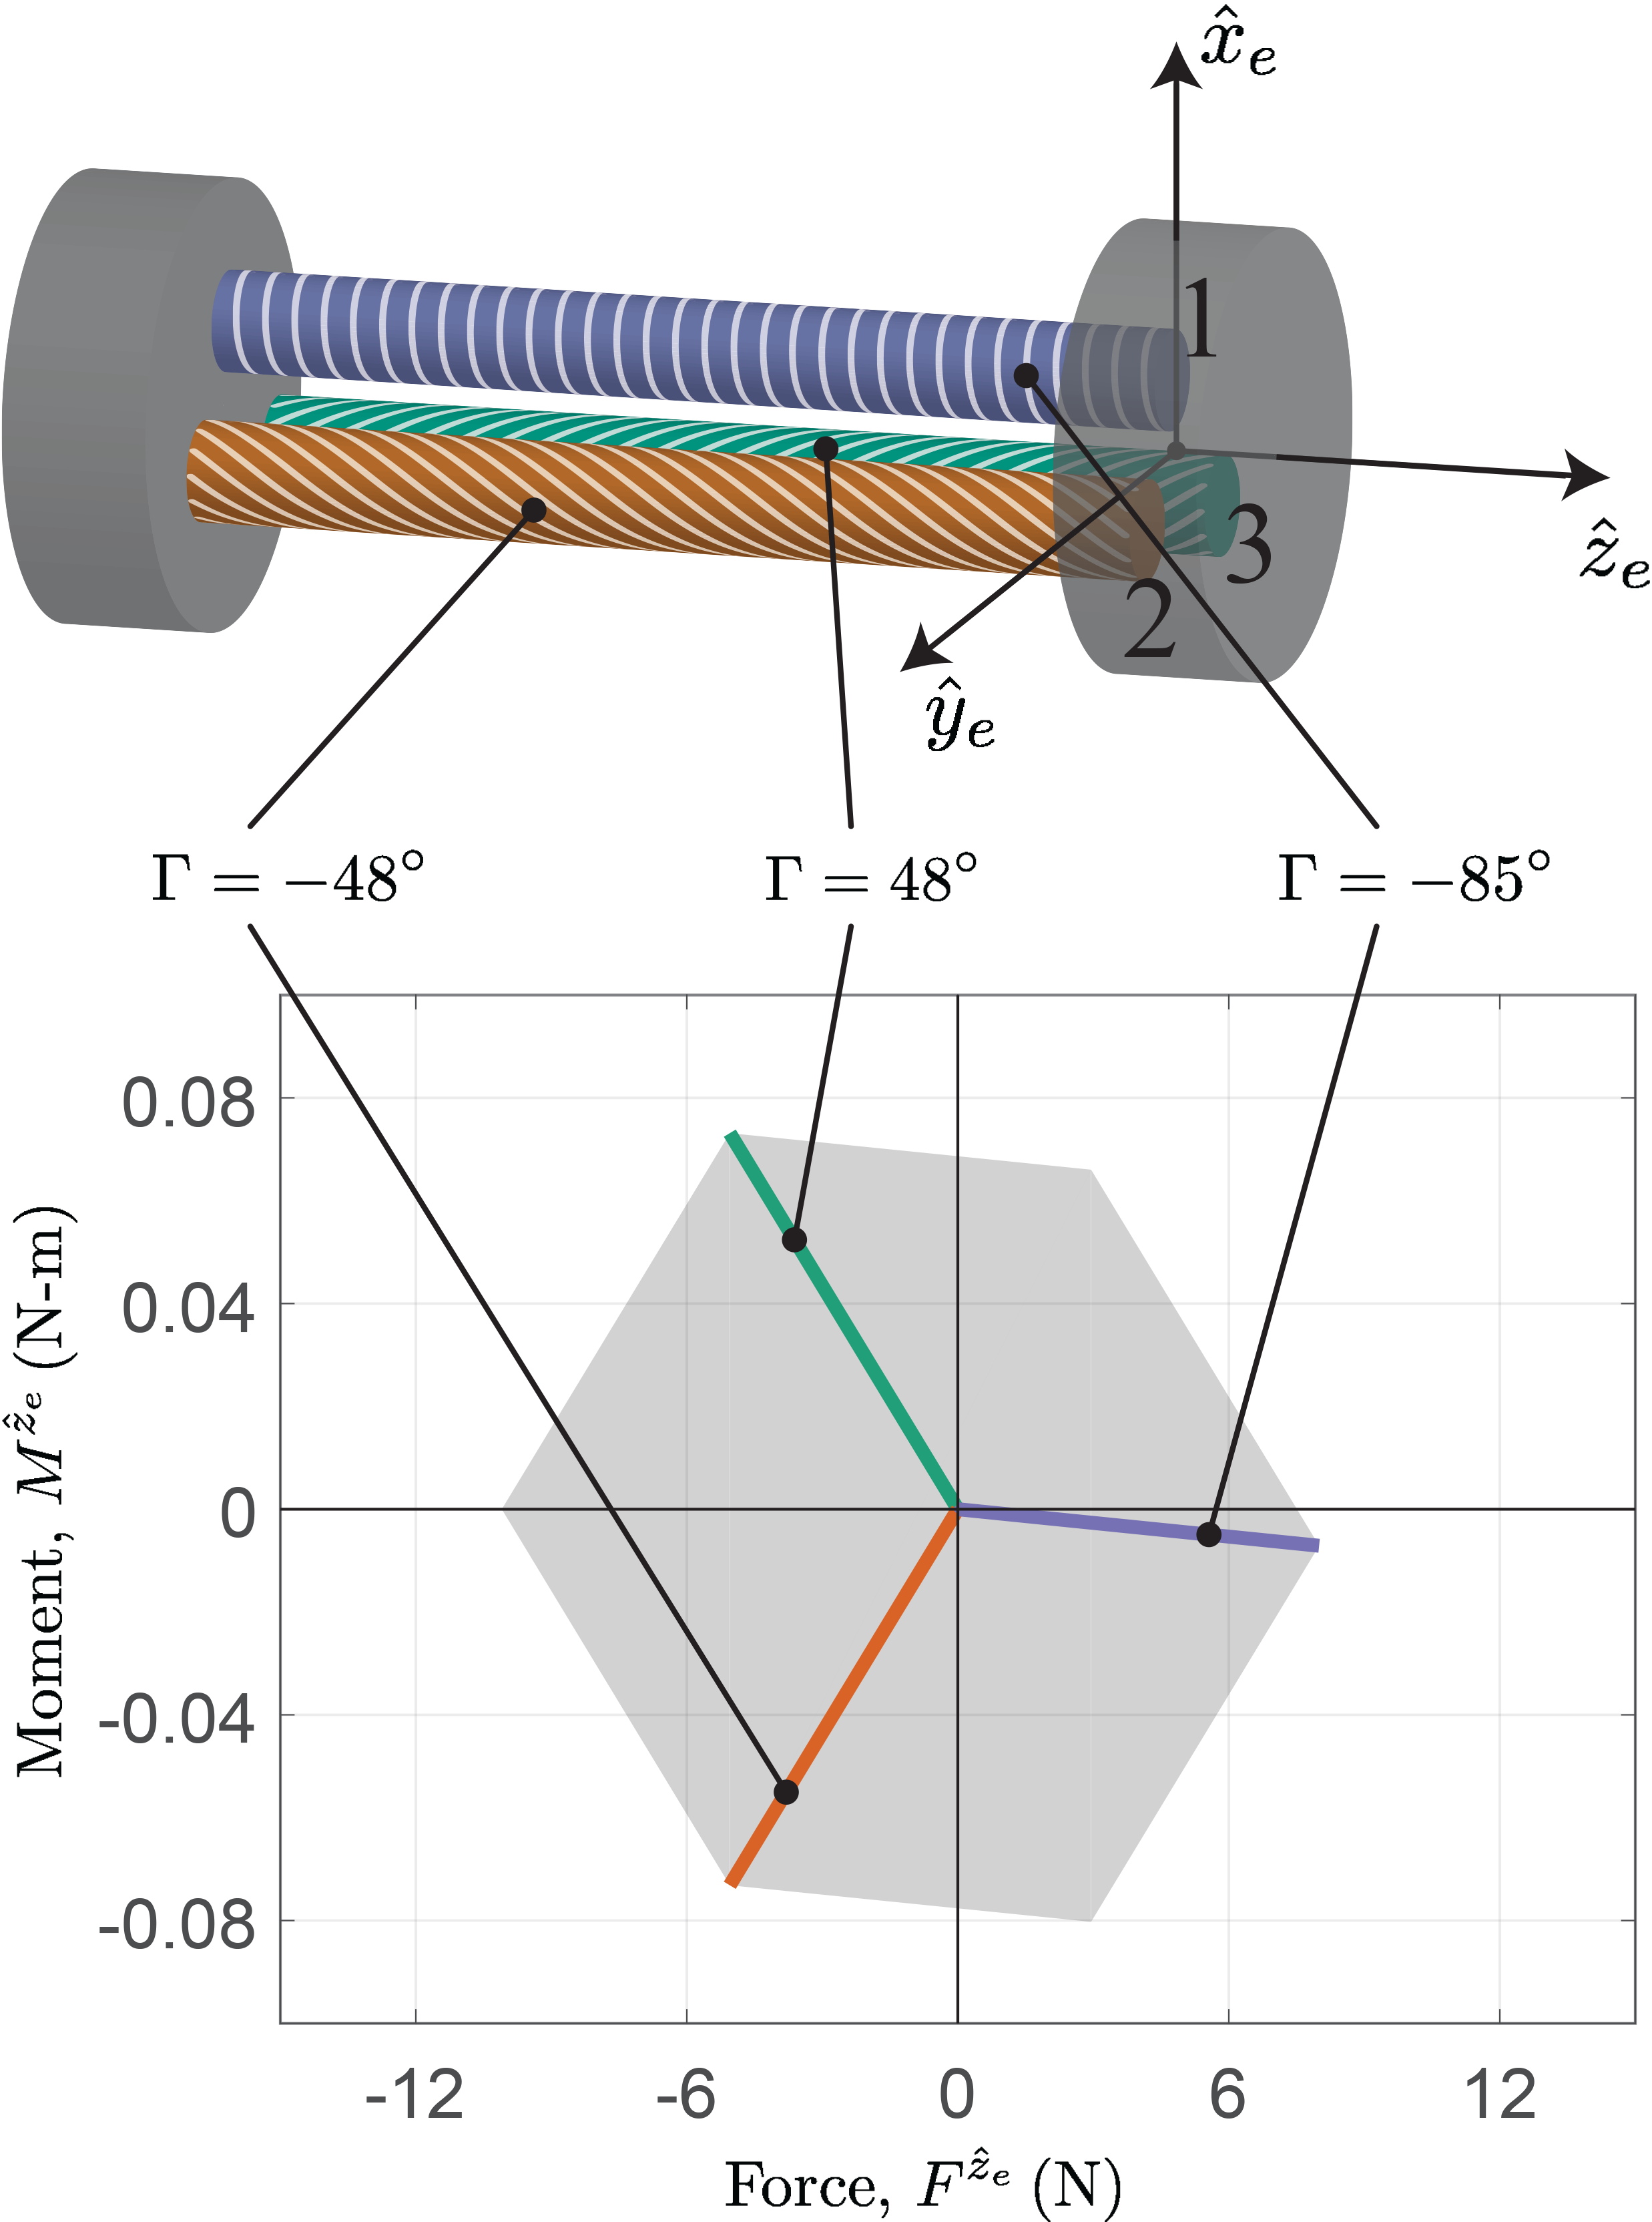
\includegraphics[width=0.85\linewidth]{figures/rigDiagram_wlabels10.png}
    \caption{In the experimental evaluation, we employed a parallel combination of three FREEs (top) to yield forces along and moments about the $z$-axis of an end effector.
    The FREEs were carefully selected to yield a well-balanced force zonotope (bottom) to gain full control authority over $F^{\hat{z}_e}$ and $M^{\hat{z}_e}$.
    To this end, we used one extending FREE, and two contracting FREEs which generate antagonistic moments about the end effector $z$-axis.}
    \label{fig:rigDiagram}
\end{figure}


\subsection{Experimental Setup}
To measure the forces generated by this actuator combination under a varying state $\vec{x}$ and pressure input $\vec{p}$, we developed a custom built test bench (Fig.~\ref{fig:rig}). 
%
\begin{figure}
    \centering
    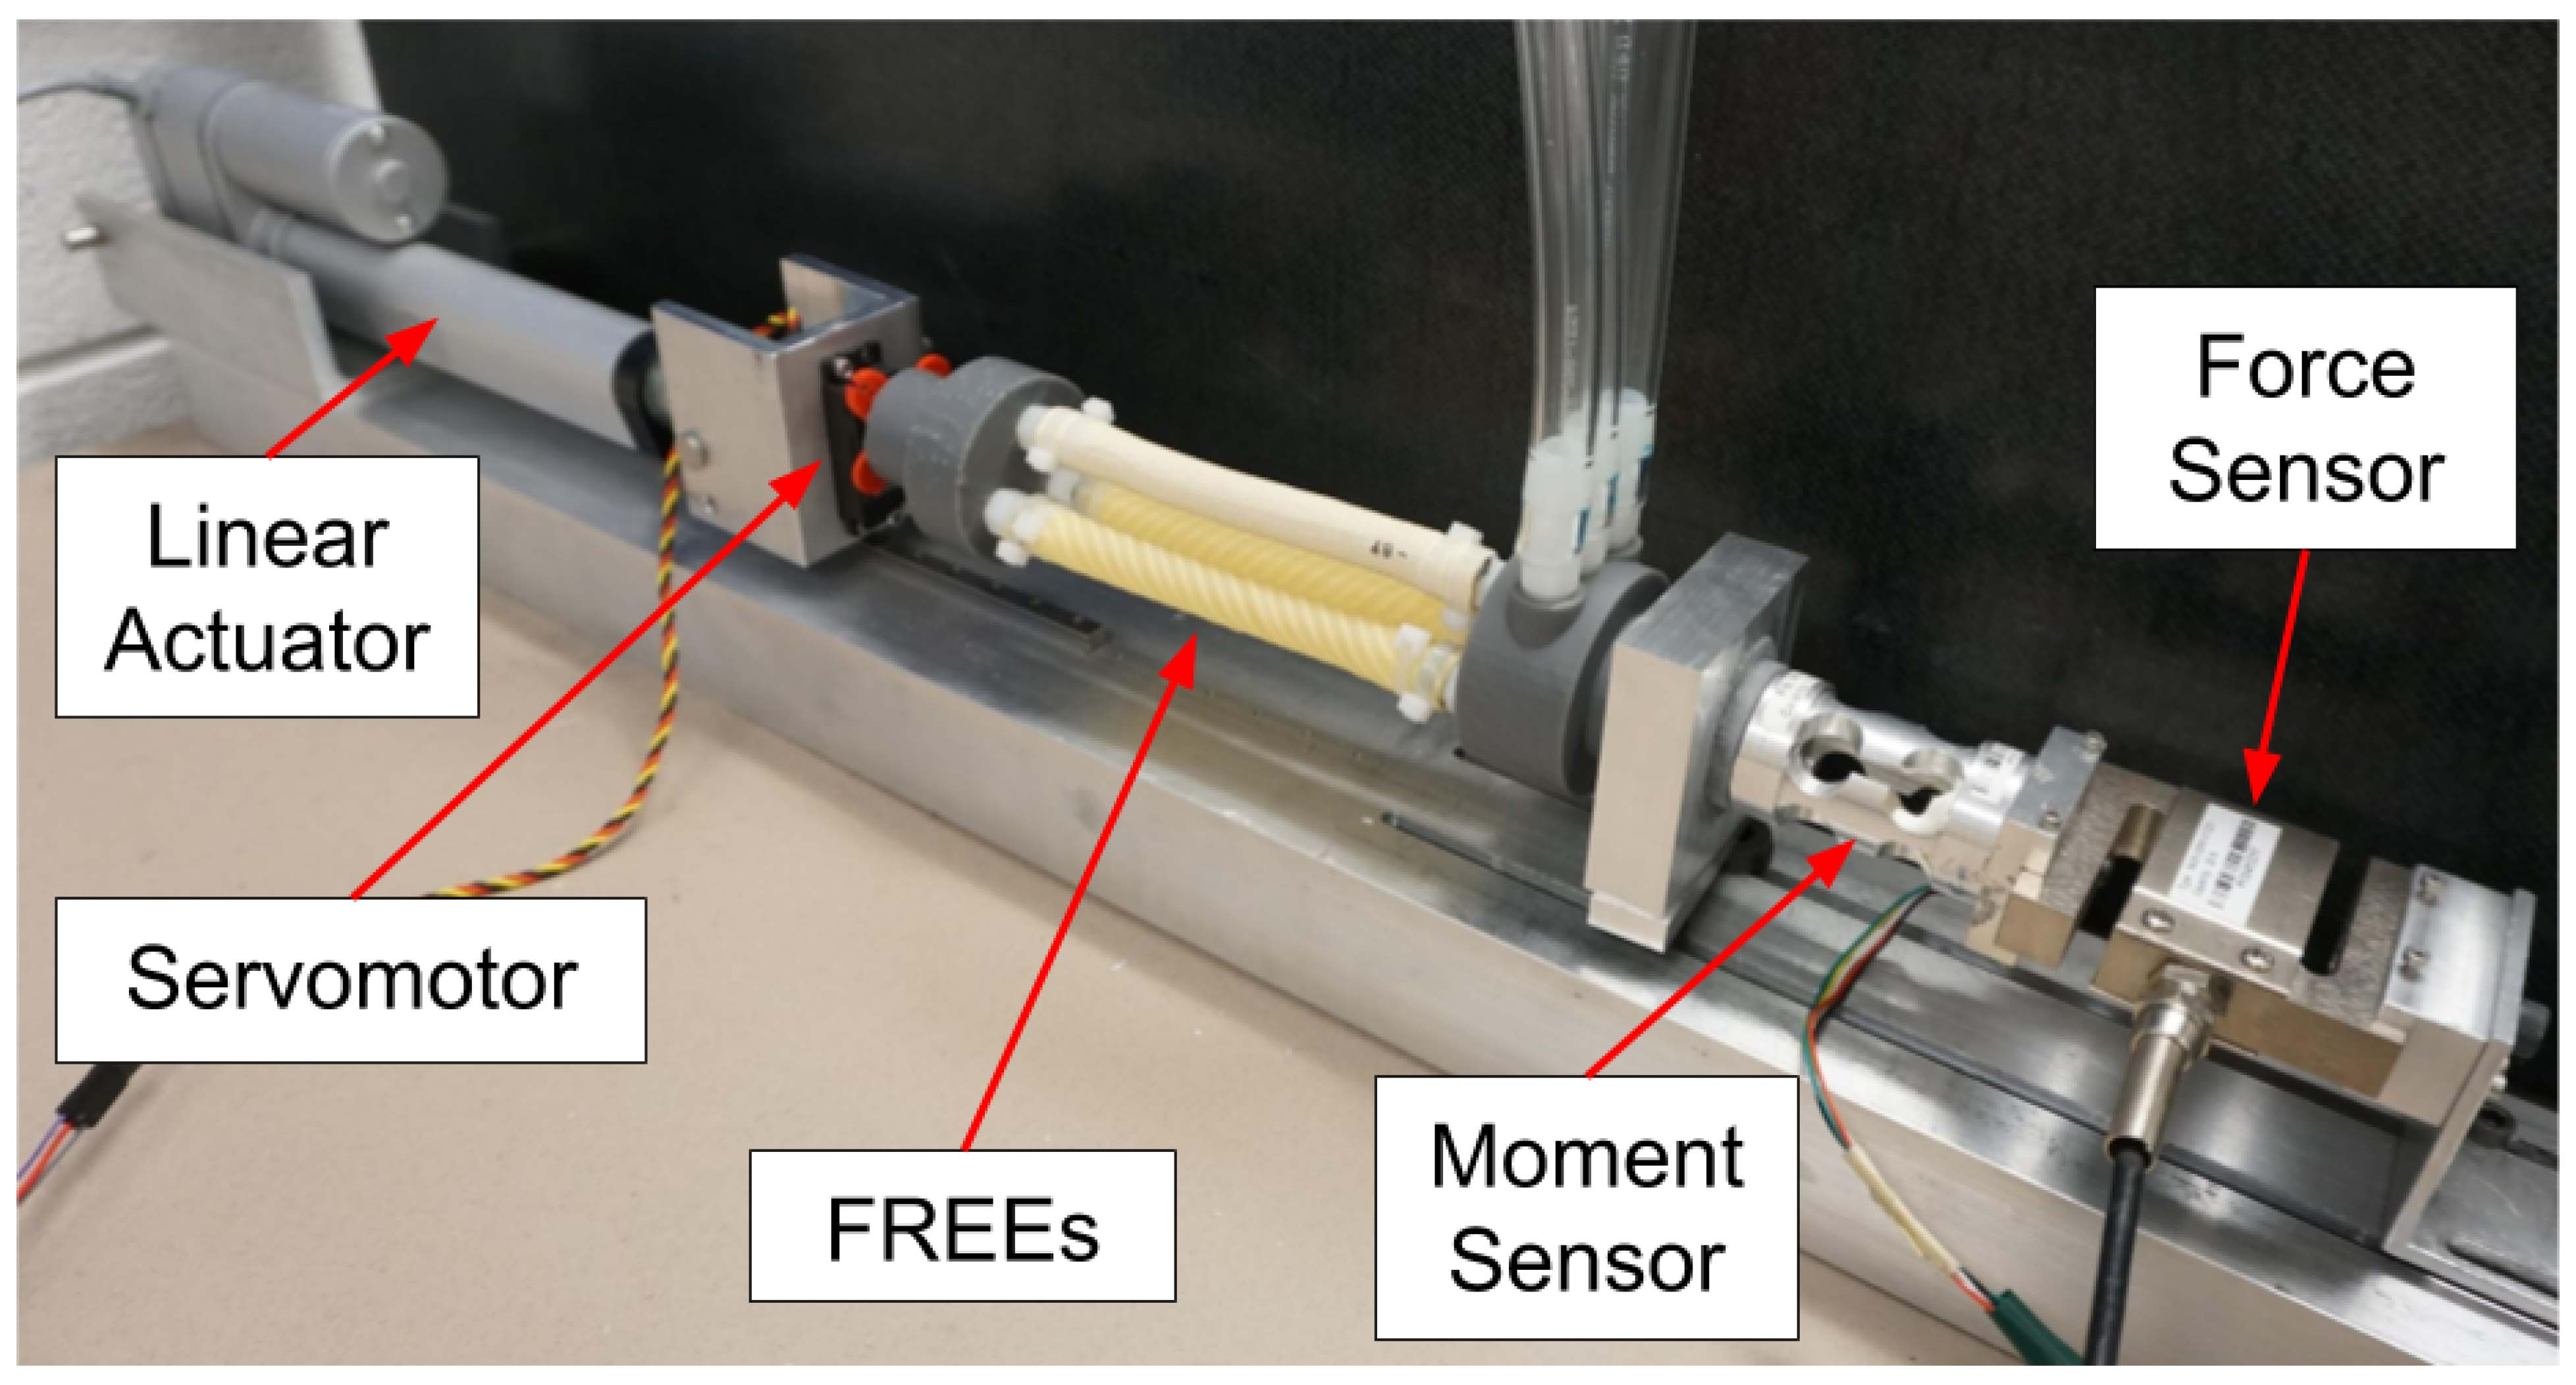
\includegraphics[width=\linewidth]{figures/photos/rig_labeled2.jpg}
    \caption{\revcomment{1.3}{This experimental rig is used to generate a targeted displacement (extension and twist) of the end effector and to measure the forces and torques created by a parallel combination of three FREEs. A linear actuator and servomotor impose an extension and a twist, respectively, while the net force and moment generated by the FREEs is measured with a force load cell and moment load cell mounted in series.}}
    \label{fig:rig}
\end{figure}
%
In the test bench, a linear actuator (ServoCity HDA 6-50) and a rotational servomotor (Hitec HS-645mg) were used to impose a 2-dimensional displacement on the end effector. 
A force load cell (LoadStar  RAS1-25lb) and a moment load cell (LoadStar RST1-6Nm) measured the end-effector forces $F^{\hat{z_e}}$ and moments $M^{\hat{z_e}}$, respectively.
During the experiments, the pressure inside the FREEs was varied using pneumatic pressure regulators (Enfield TR-010-g10-s). 

The FREE attachment points (measured from the end effector origin) were measured to be:
\begin{align}
    \vec{d}_1 &= \bmx 0.013 & 0 & 0 \emx^T  \text{m}\\
    \vec{d}_2 &= \bmx -0.006 & 0.011 & 0 \emx^T  \text{m}\\
    \vec{d}_3 &= \bmx -0.006 & -0.011 & 0 \emx^T \text{m}
%    \vec{d}_i &= \bmx 0 & 0 & 0 \emx^T , && \text{for } i = 1,2,3
\end{align}
All three FREEs were oriented parallel to the end effector $z$-axis:
\begin{align}
    \hat{a}_i &= \bmx 0 & 0 & 1 \emx^T, \hspace{20pt} \text{for } i = 1,2,3
\end{align}
Based on this geometry, the transformation matrices $\bar{\mathcal{D}}_i$ were given by:
\begin{align}
    \bar{\mathcal{D}}_1 &= \bmx 0 & 0 & 1 & 0 & -0.013 & 0 \\ 0 & 0 & 0 & 0 & 0 & 1 \emx^T  \\
    \bar{\mathcal{D}}_2 &= \bmx 0 & 0 & 1 & 0.011 & 0.006 & 0 \\ 0 & 0 & 0 & 0 & 0 & 1 \emx^T  \\
    \bar{\mathcal{D}}_3 &= \bmx 0 & 0 & 1 & -0.011 & 0.006 & 0 \\ 0 & 0 & 0 & 0 & 0 & 1 \emx^T 
%    \bar{\mathcal{D}}_i &= \bmx 0 & 0 & 1 & 0 & 0 & 0 \\ 0 & 0 & 0 & 0 & 0 & 1 \emx^T , && \text{for } i = 1,2,3
\end{align}
These matrices were used in equation \eqref{eq:zeta} to yield the state-dependent fluid Jacobian $\bar{J}_x$ and to compute the resulting force zontopes.
%while using measured values of $\vec{\zeta}^{\,\text{meas}} (\vec{q}, \vec{P})$ and $\vec{\zeta}^{\,\text{meas}} (\vec{q}, 0)$ in \eqref{eq:fiberIso} yields the empirical measurements of the active force.



\subsection{Isolating the Active Force}
In order to compare our model force predictions (which focus only on the active forces induced by the fibers)
to those measured empirically on a physical system, we had to remove the elastic force components attributed to the elastomer. 
Under the assumption that the elastomer force is merely a function of the displacement $\vec{x}$ and independent of pressure $\vec{p}$ \cite{bruder2017model}, this force component can be approximated by the measured force at a pressure of $\vec{p}=0$. 
That is: 
\begin{align}
    \vec{f}_{\text{elast}} (\vec{x}) = \vec{f}_{\text{\,meas}} (\vec{x}, 0)
\end{align}
With this, the active generalized forces can be measured indirectly by subtracting off the force generated at zero pressure:
\begin{align}
    \vec{f} (\vec{x}, \vec{p})  &= \vec{f}_{\text{meas}} (\vec{x}, \vec{p}) - \vec{f}_{\text{meas}} (\vec{x}, 0)     \label{eq:fiberIso}
\end{align}


%To validate our parallel force model, we compare its force predictions, $\vec{\zeta}_{\text{pred}}$, to those measured empirically on a physical system, $\vec{\zeta}_\text{meas}$. 
%From \eqref{eq:Z} and \eqref{eq:zeta}, the force at the end effector is given by:
%\begin{align}
%    \vec{\zeta}(\vec{q}, \vec{P}) &= \sum_{i=1}^n \bar{\mathcal{D}}_i \left( {\bar{J}_V}_i^T(\vec{q_i}) P_i + \vec{Z}_i^{\text{elast}} (\vec{q_i}) \right) \\
%    &= \underbrace{\sum_{i=1}^n \bar{\mathcal{D}}_i {\bar{J}_V}_i^T(\vec{q_i}) P_i}_{\vec{\zeta}^{\,\text{fiber}} (\vec{q}, \vec{P})} + \underbrace{\sum_{i=1}^n \bar{\mathcal{D}}_i \vec{Z}_i^{\text{elast}} (\vec{q_i})}_{\vec{\zeta}^{\text{elast}} (\vec{q})}   \label{eq:zetaSplit}
%     &= \vec{\zeta}^{\,\text{fiber}} (\vec{q}, \vec{P}) + \vec{\zeta}^{\text{elast}} (\vec{q})
%\end{align}
%\Dan{These will need to reflect changes made to previous section.}
%The model presented in this paper does not specify the elastomer forces, $\vec{\zeta}^{\text{elast}}$, therefore we only validate its predictions %of the fiber forces, $\vec{\zeta}^{\,\text{fiber}}$. 
%We isolate the fiber forces by noting that $\vec{\zeta}^{\text{elast}} (\vec{q}) = \vec{\zeta}(\vec{q}, 0)$ and rearranging \eqref{eq:zetaSplit}
%\begin{align}
%    \vec{\zeta}^{\,\text{fiber}} (\vec{q}, \vec{P})  &= \vec{\zeta}(\vec{q}, \vec{P}) - \vec{\zeta}(\vec{q}, 0)     \label{eq:fiberIso}
%%    \vec{\zeta}^{\,\text{fiber}}_{\text{emp}} (\vec{q}, \vec{P})  &= \vec{\zeta}_{\text{emp}}(\vec{q}, \vec{P}) - %\vec{\zeta}_{\text{emp}}(\vec{q}, 0)
%\end{align}
%Thus we measure the fiber forces indirectly by subtracting off the forces generated at zero pressure.  


\subsection{Experimental Protocol}
The force and moment about the end effector $z$-axis generated by the parallel combination FREEs was measured in four different geometric configurations: neutral, extended, twisted, and simultaneously extended and twisted (see Table \ref{table:RMSE} for the exact deformation amounts). 
At each of these configurations, the forces were measured at all pressure combinations in the set
\begin{align}
    \mathcal{P} &= \left\{ \bmx \alpha_1 & \alpha_2 & \alpha_3 \emx^T p^{\text{max}} \, : \, \alpha_i = \left\{ 0, \frac{1}{4}, \frac{1}{2}, \frac{3}{4}, 1 \right\} \right\}
\end{align}
with $p^{\text{max}}$ = \unit[103.4]{kPa}. 



\subsection{Results}

\begin{figure*}[h]
\centering

\def\picScale{0.08}    % define variable for scaling all pictures evenly
\def\plotScale{0.2}    % define variable for scaling all plots evenly
\def\colWidth{0.22\linewidth}

\begin{tikzpicture} %[every node/.style={draw=black}]
% \draw[help lines] (0,0) grid (4,2);
\matrix [row sep=0cm, column sep=0cm, style={align=center}] (my matrix) at (0,0) %(2,1)
{
& \node (q1) {(a) $\Delta l = 0, \Delta \phi = 0$}; & \node (q2) {(b) $\Delta l = 5\text{mm}, \Delta \phi = 0$}; & \node (q3) {(c) $\Delta l = 0, \Delta \phi = 20^\circ$}; & \node (q4) {(d) $\Delta l = 5\text{mm}, \Delta \phi = 20^\circ$};

\\

&
\node[style={anchor=center}] {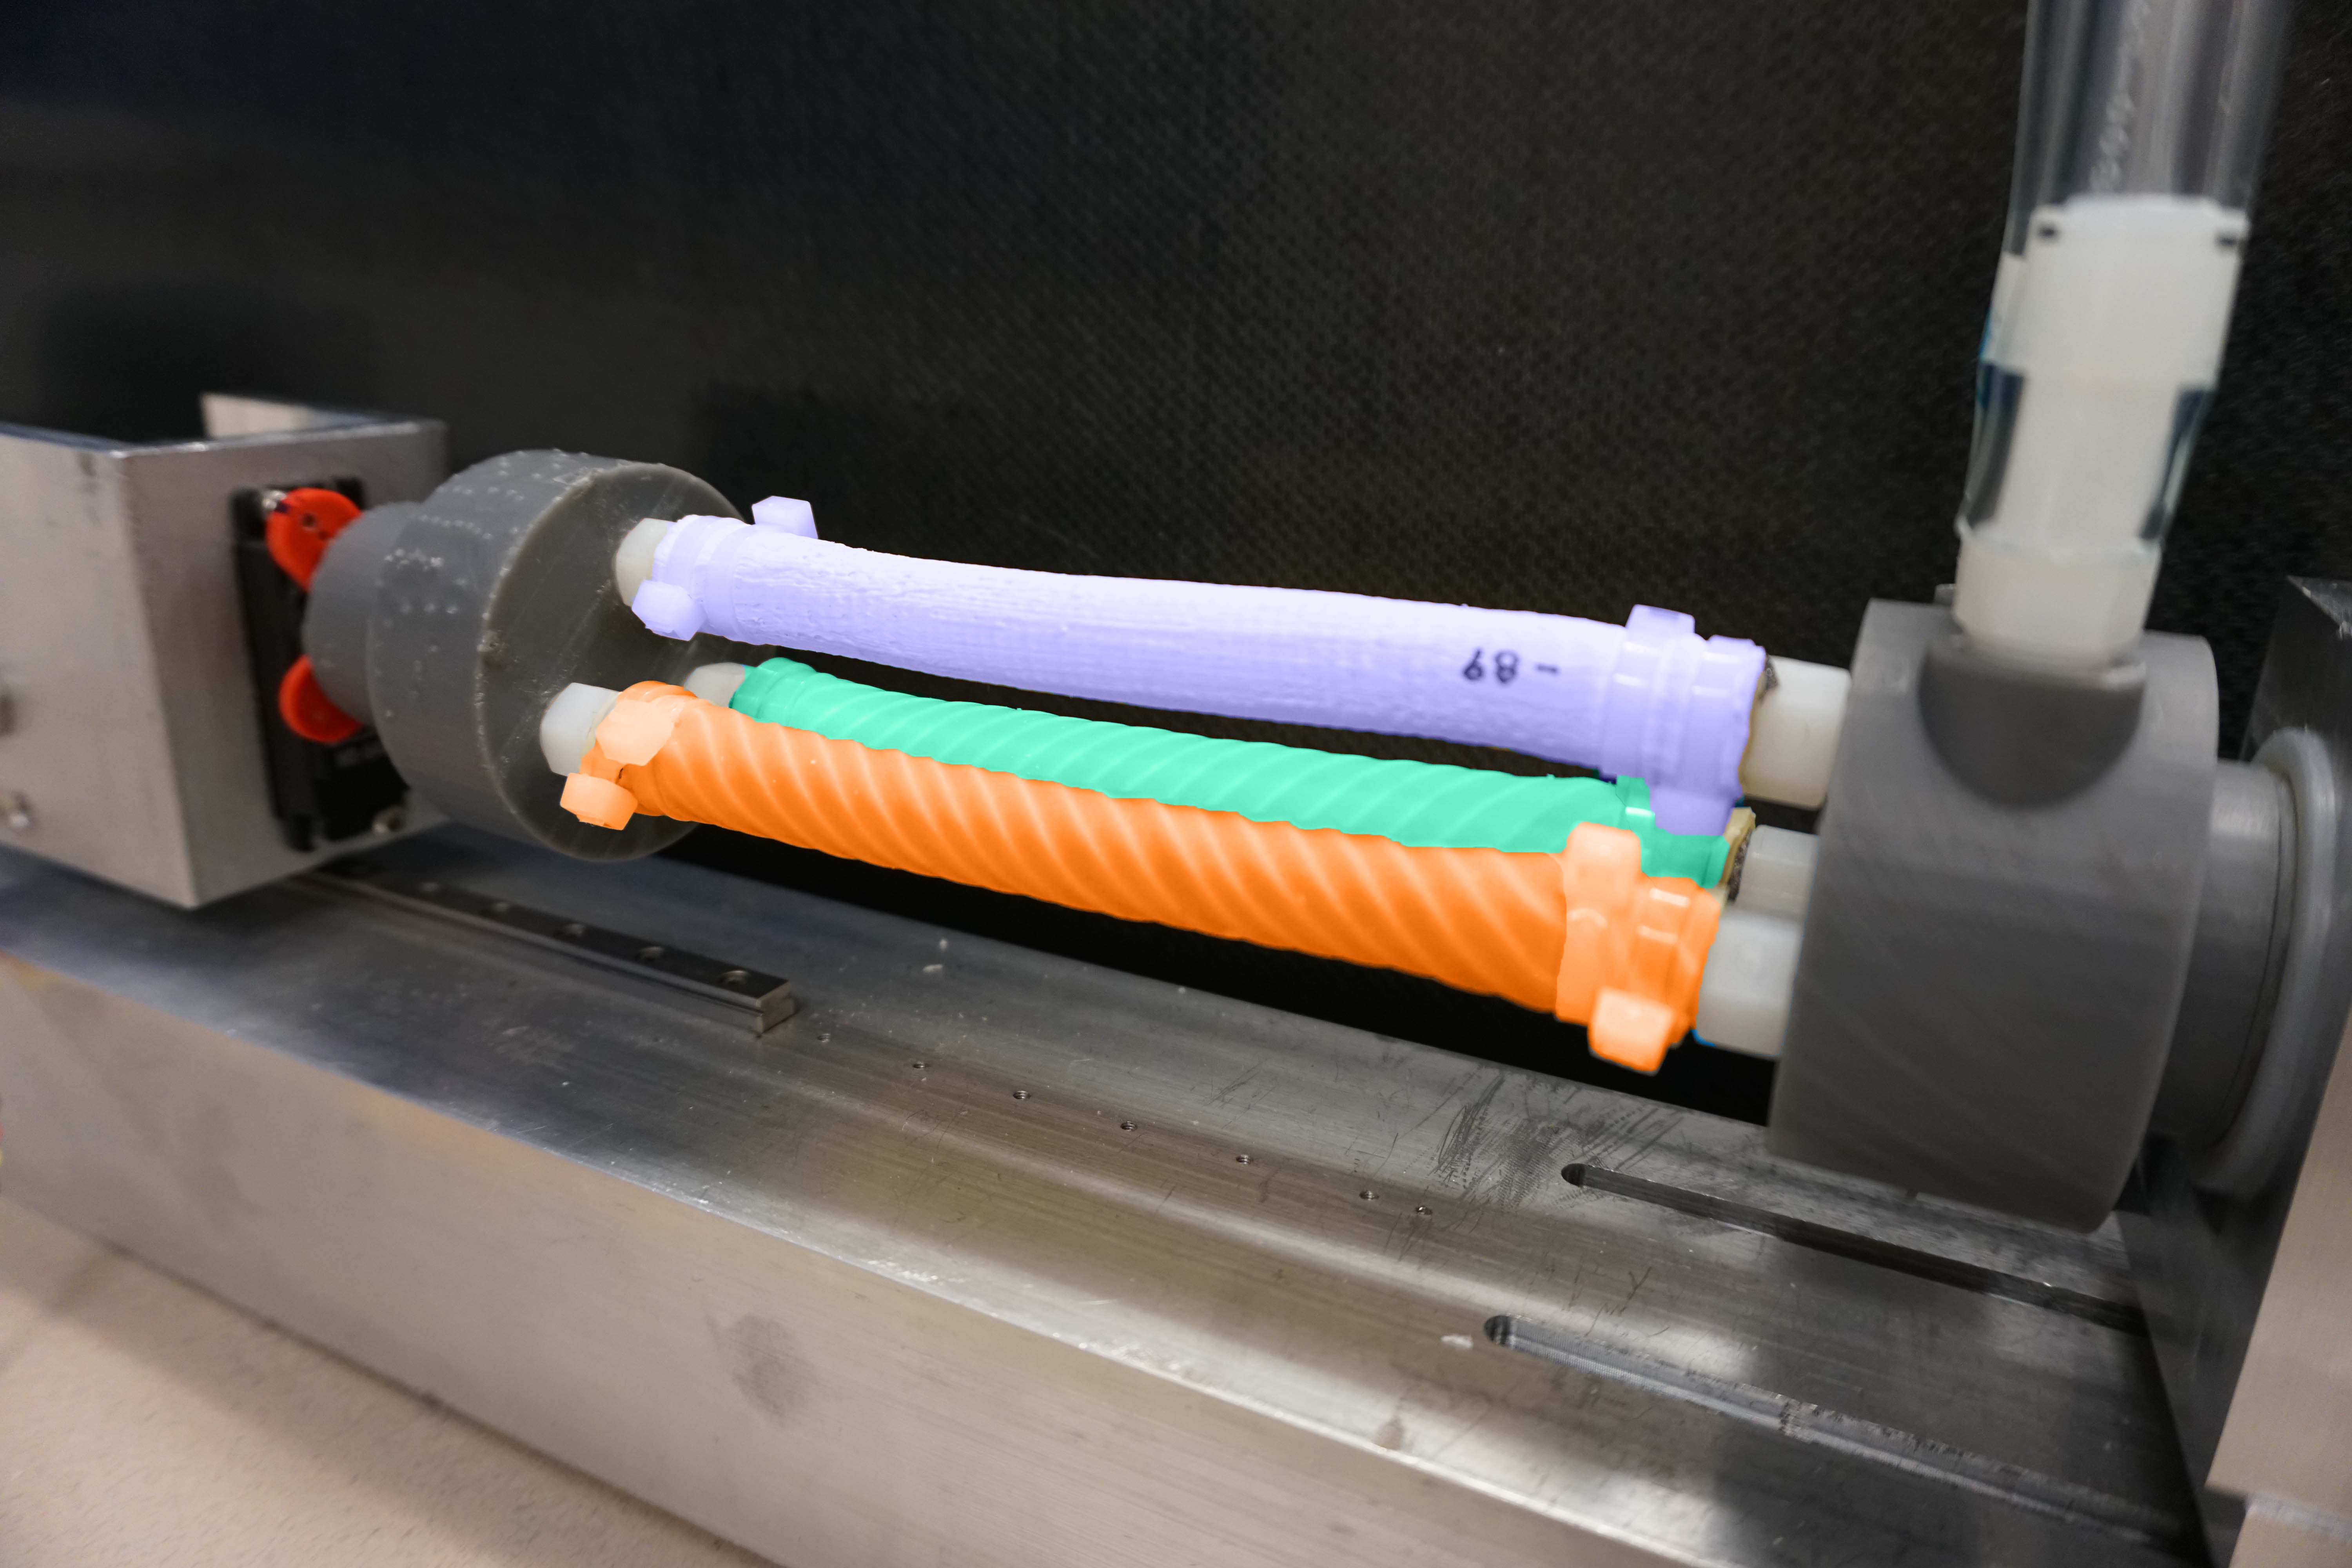
\includegraphics[width=\colWidth]{figures/photos/s0w0pic_colored.jpg}}; %\fill[blue] (0,0) circle (2pt);
&
\node[style={anchor=center}] {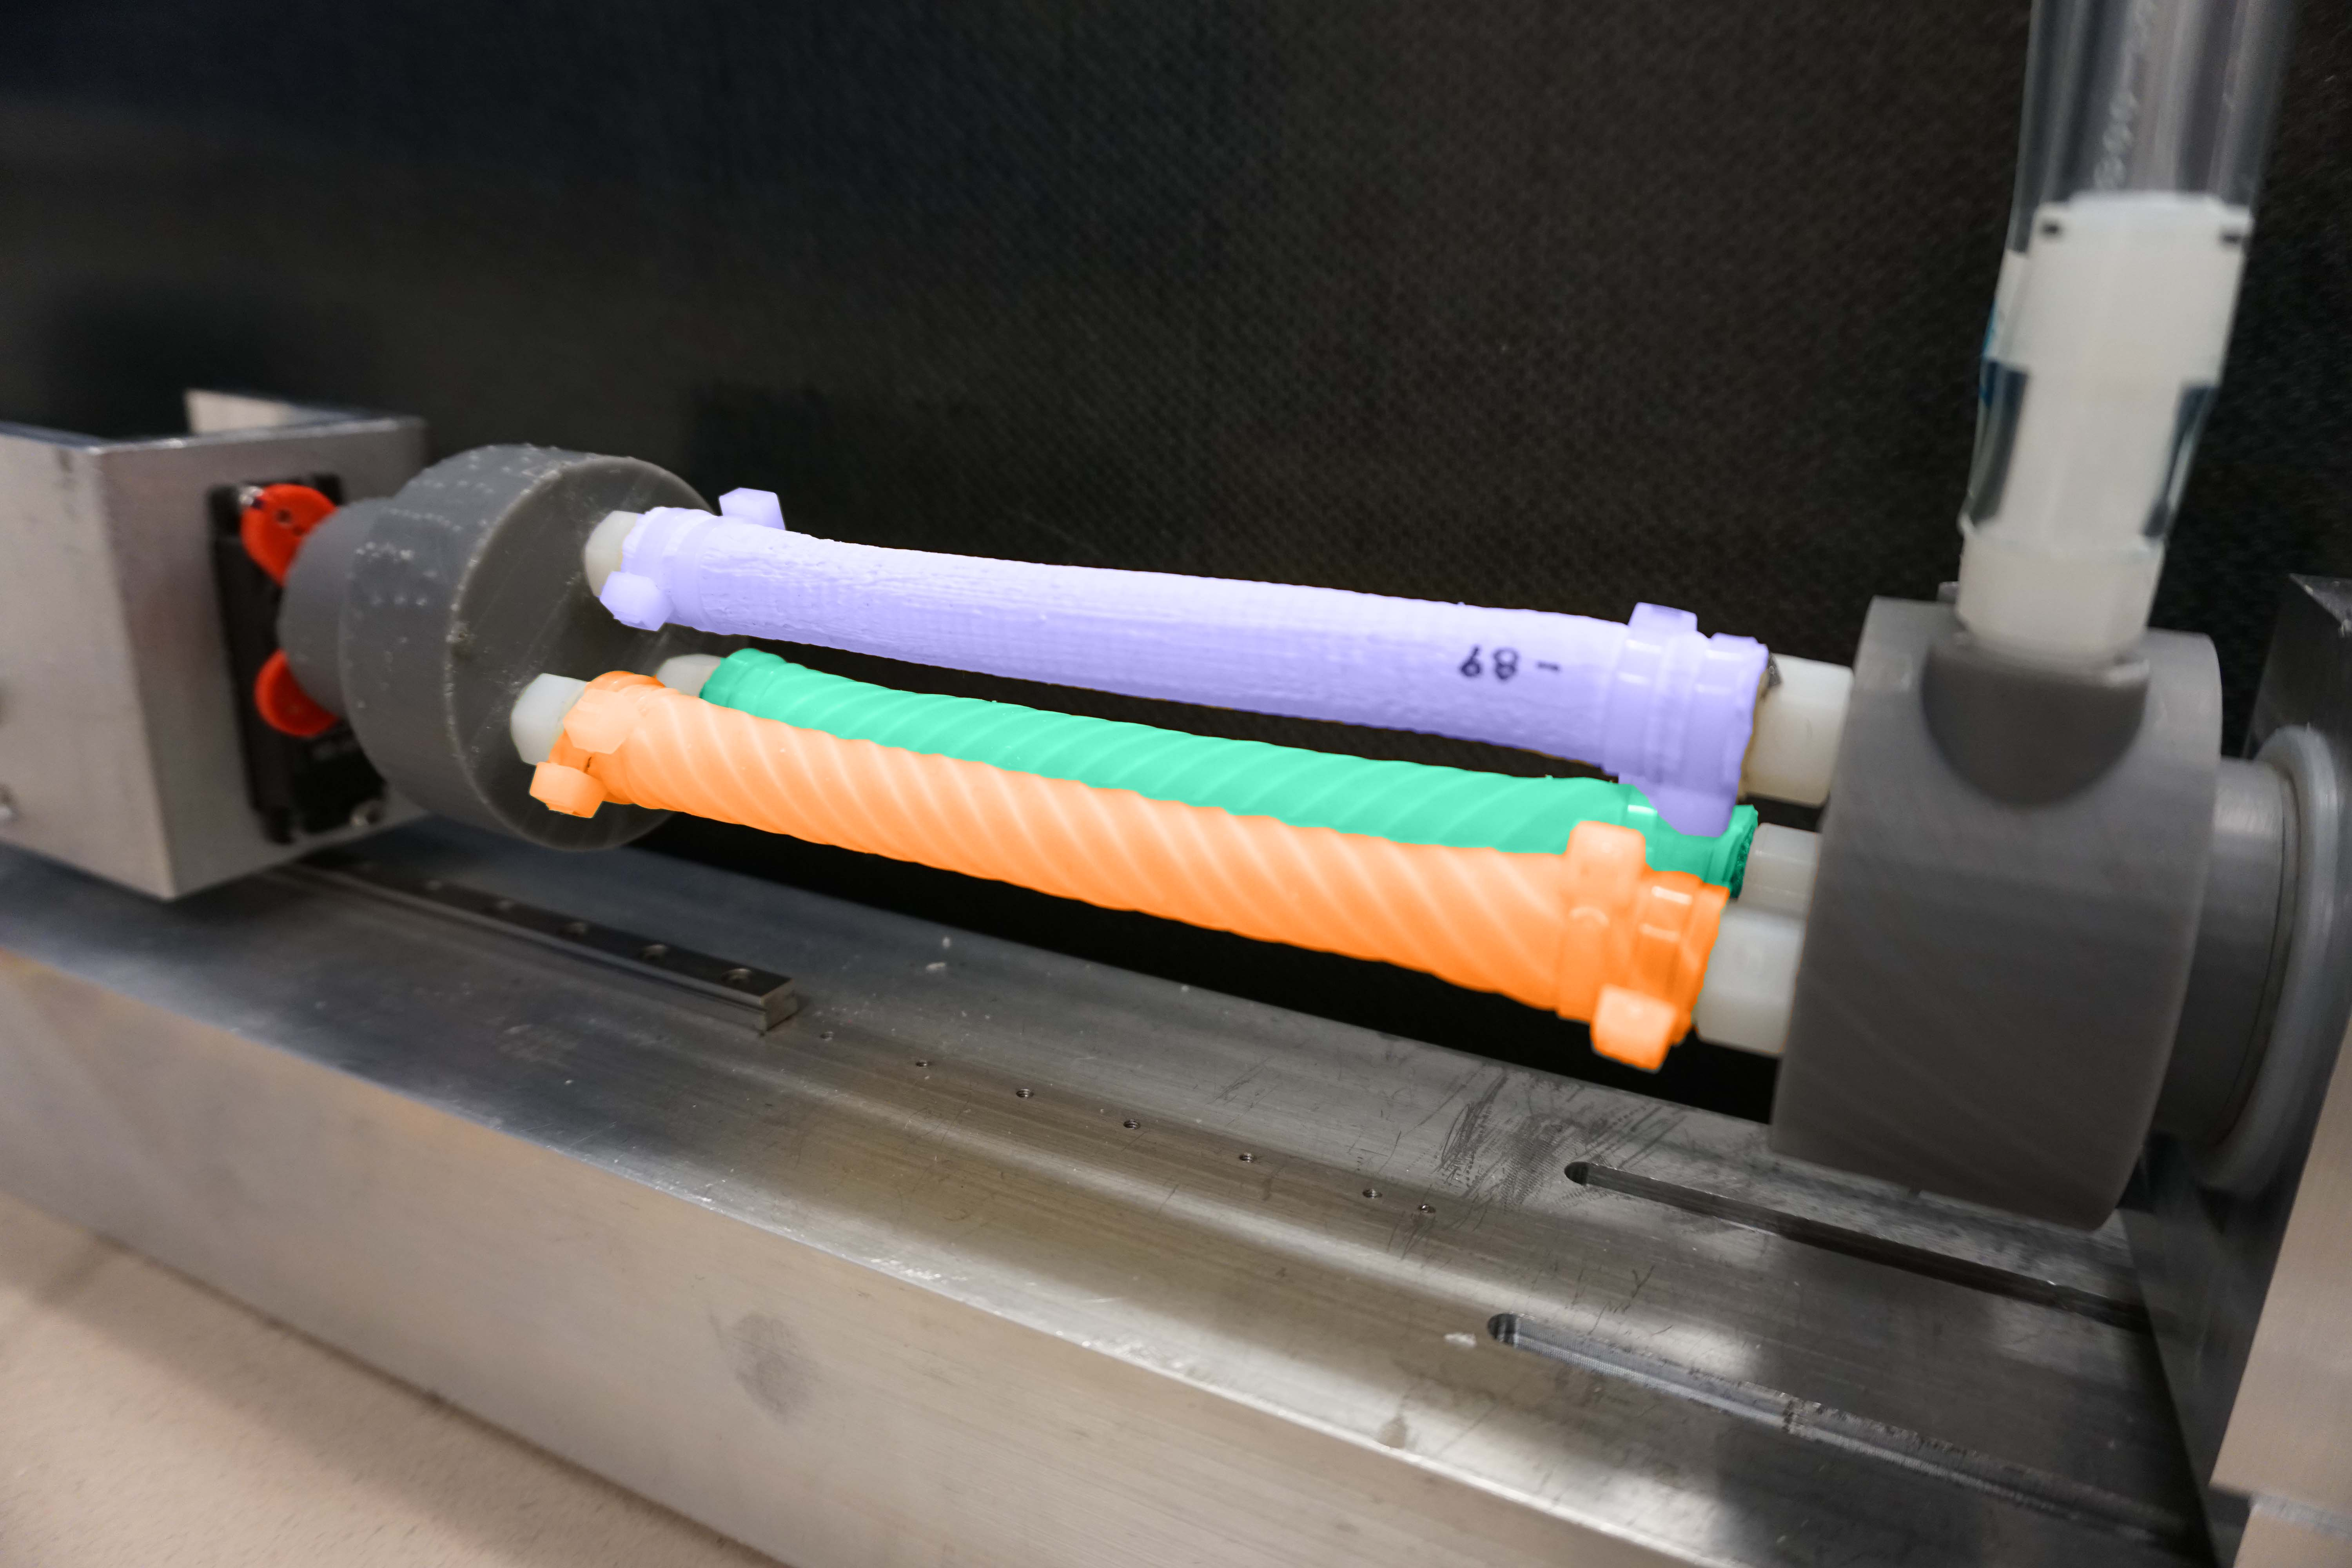
\includegraphics[width=\colWidth]{figures/photos/s5w0pic_colored.jpg}}; %\fill[blue] (0,0) circle (2pt);
&
\node[style={anchor=center}] {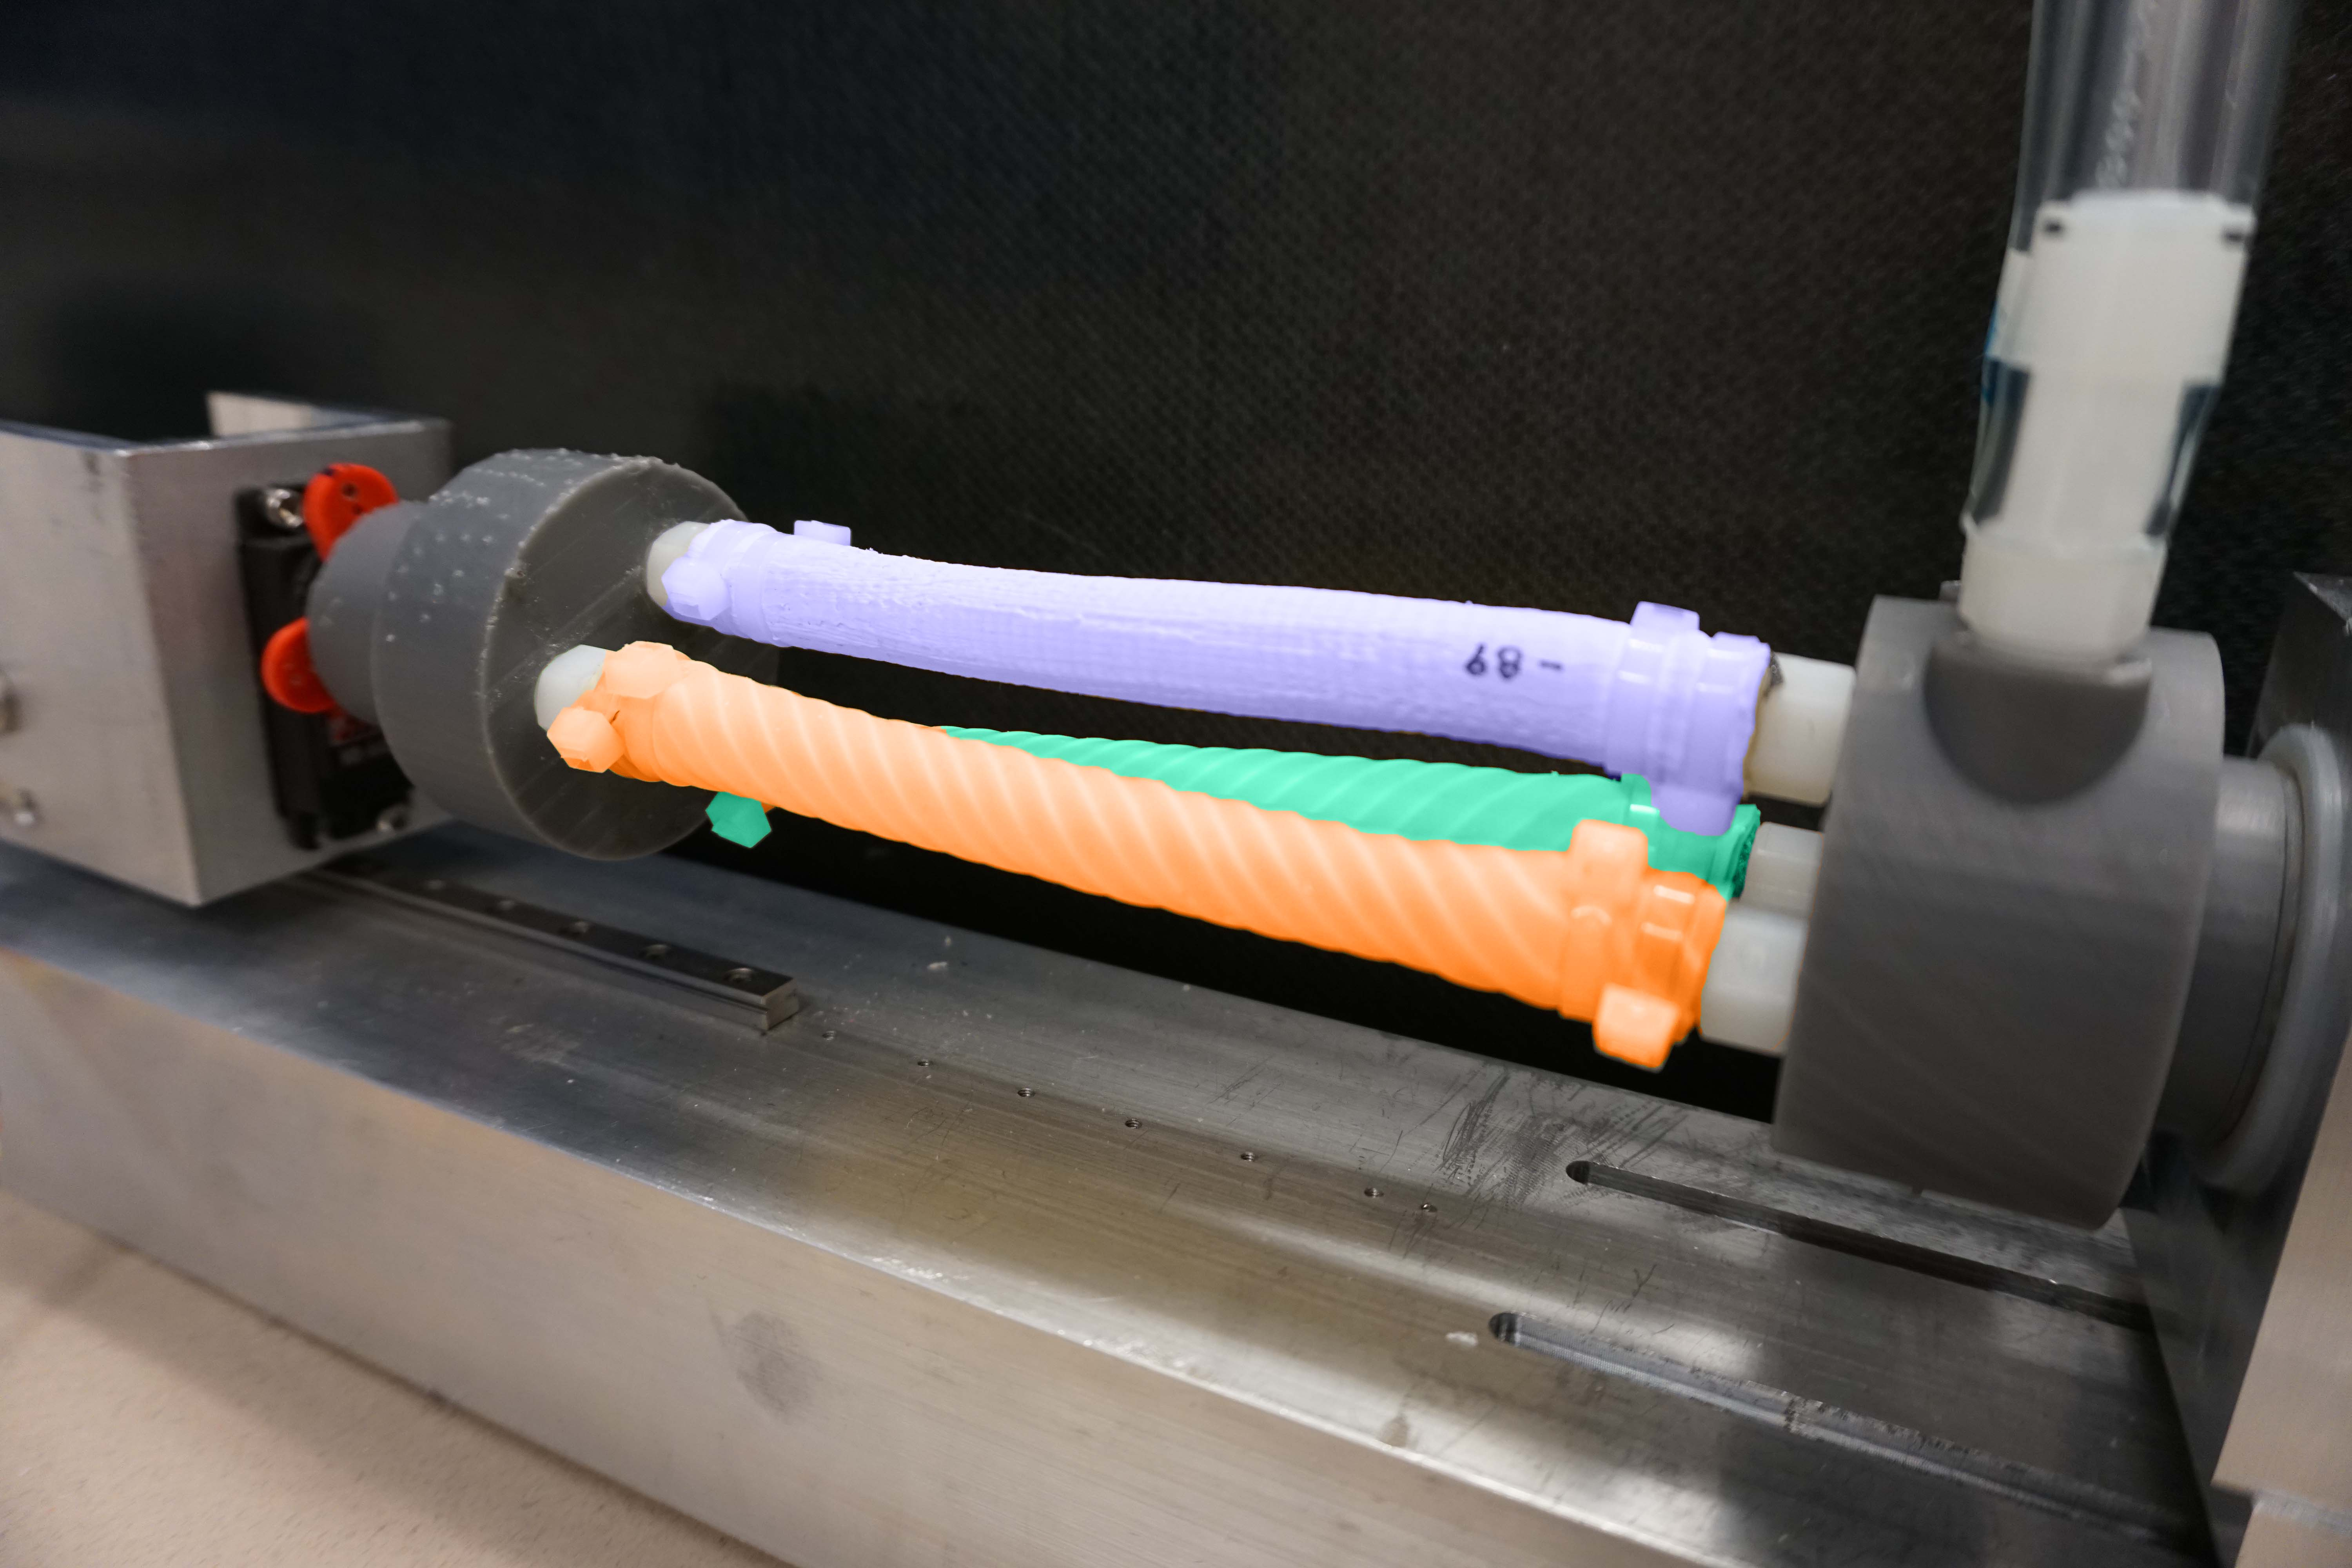
\includegraphics[width=\colWidth]{figures/photos/s0w20pic_colored.jpg}}; %\fill[blue] (0,0) circle (2pt);
&
\node[style={anchor=center}] {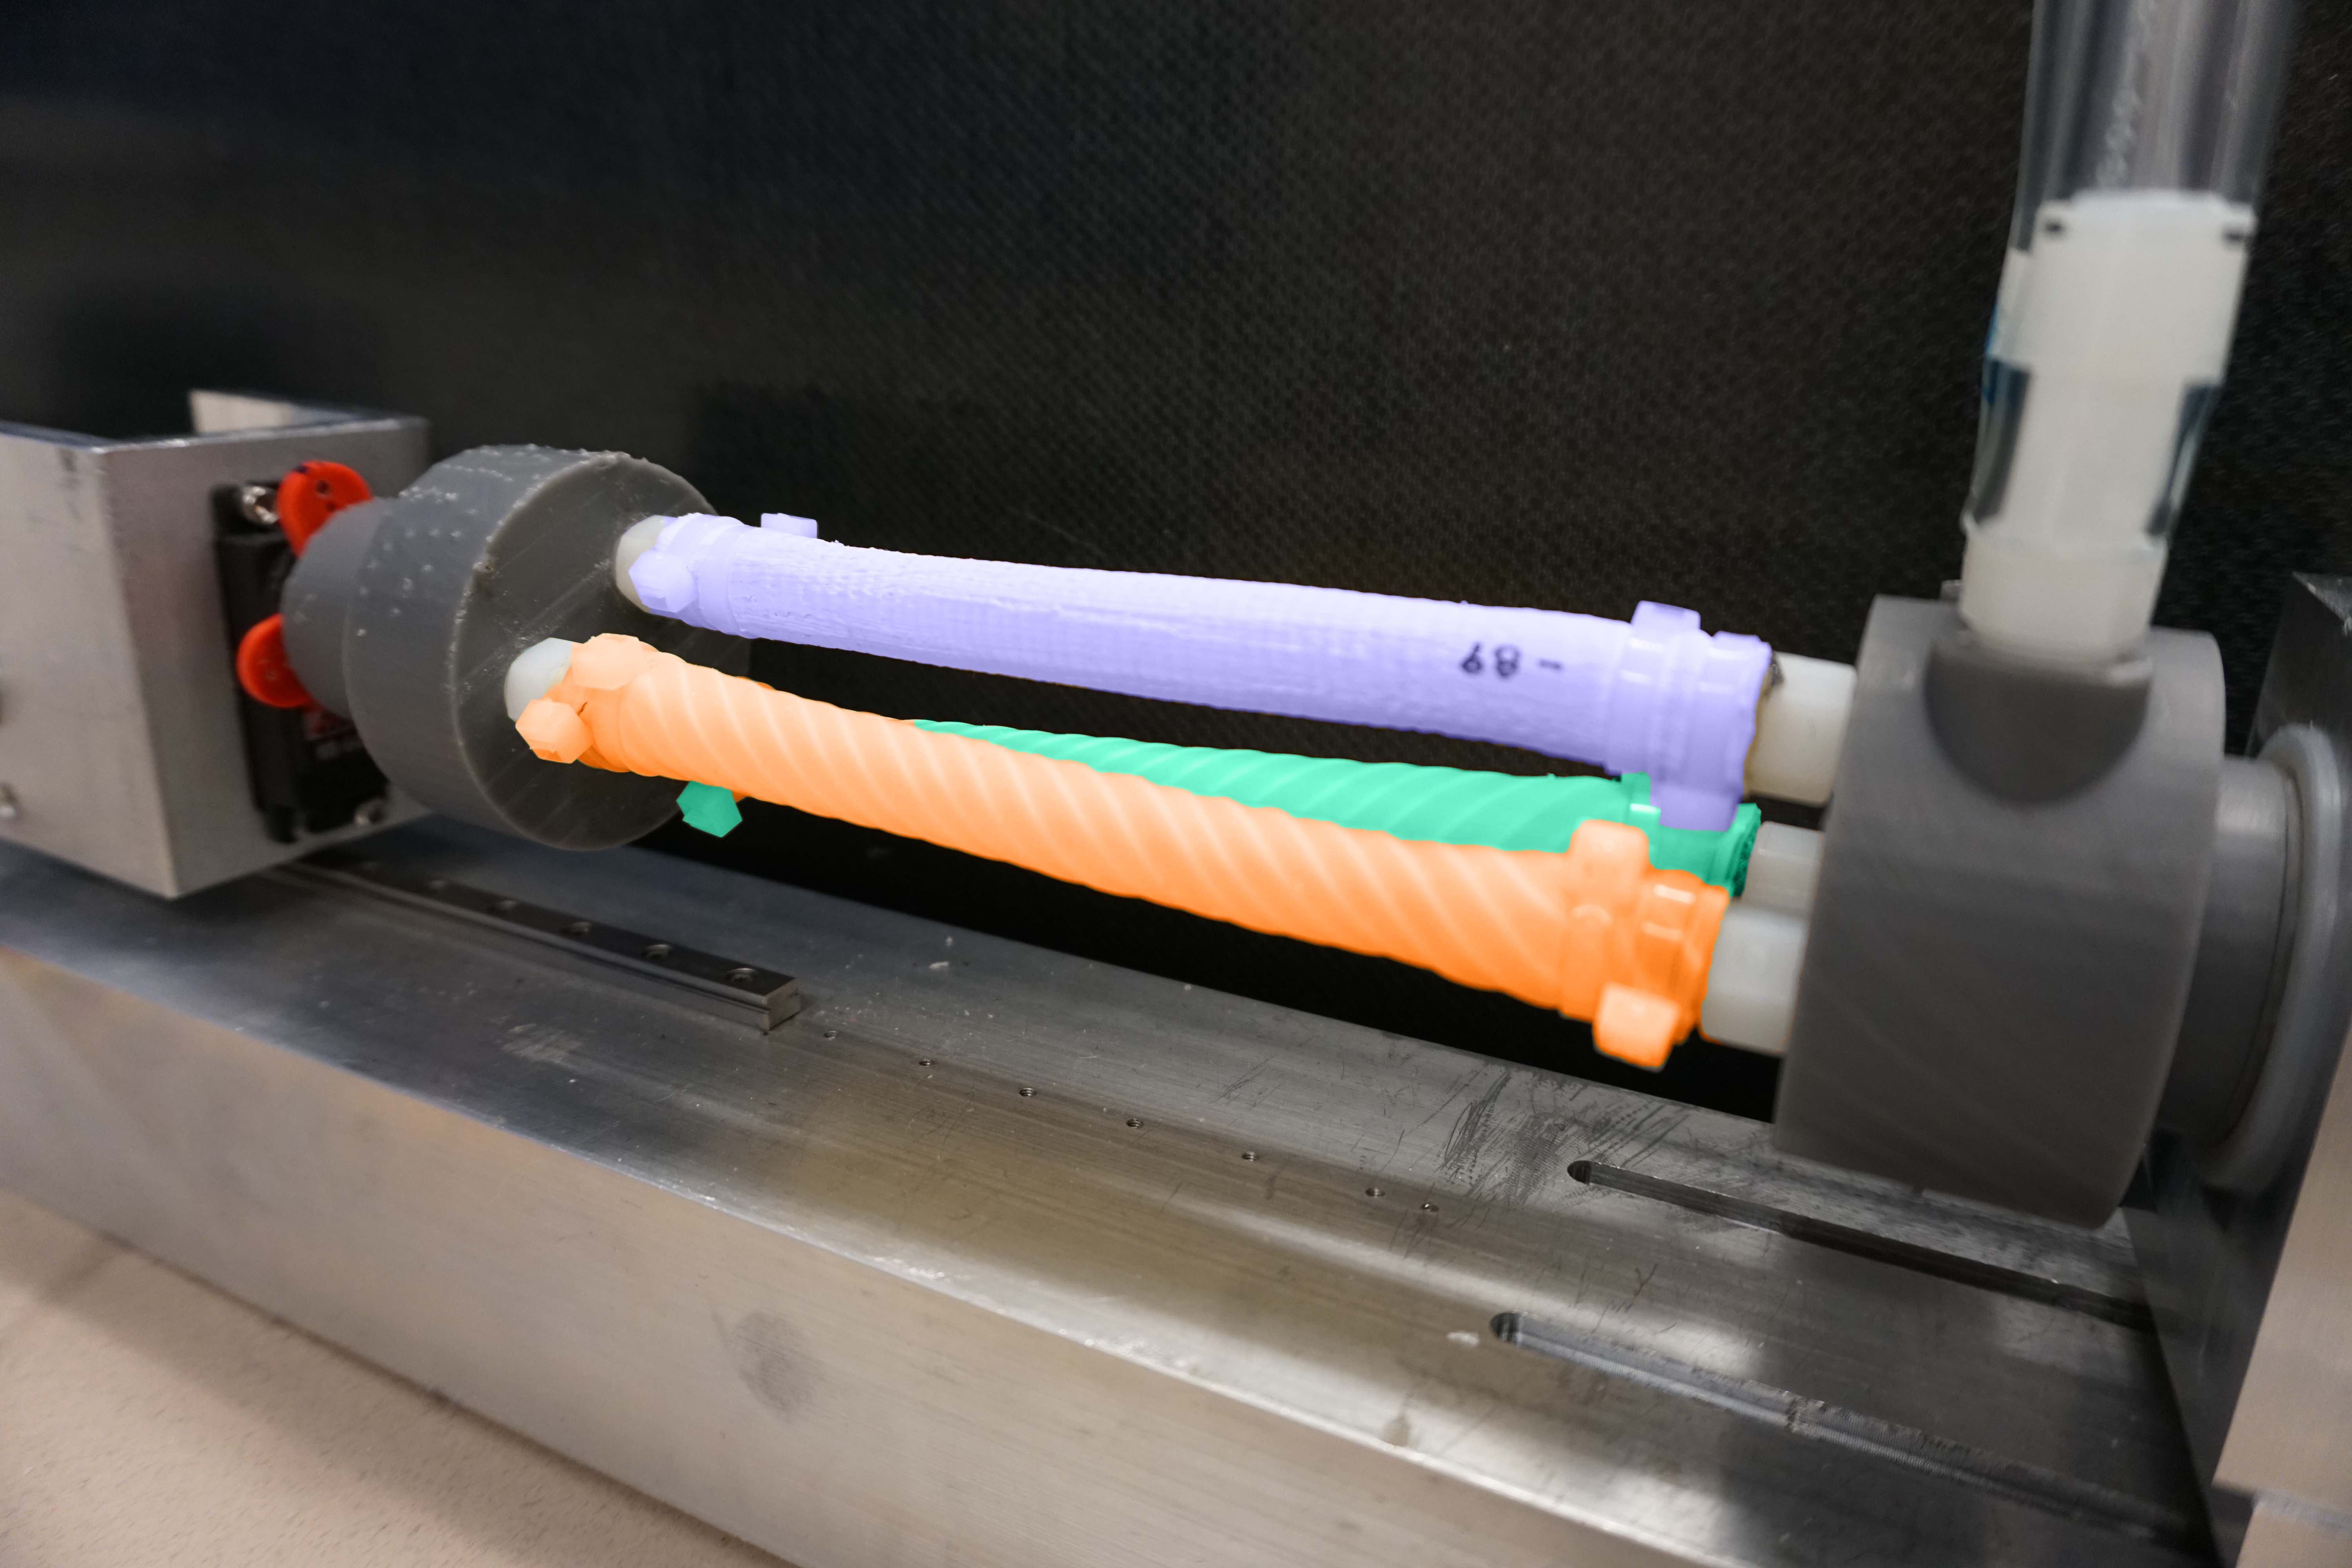
\includegraphics[width=\colWidth]{figures/photos/s5w20pic_colored.jpg}}; %\fill[blue] (0,0) circle (2pt);

\\

\node[rotate=90] (ylabel) {Moment, $M^{\hat{z}_e}$ (N-m)};
&
\node[style={anchor=center}] {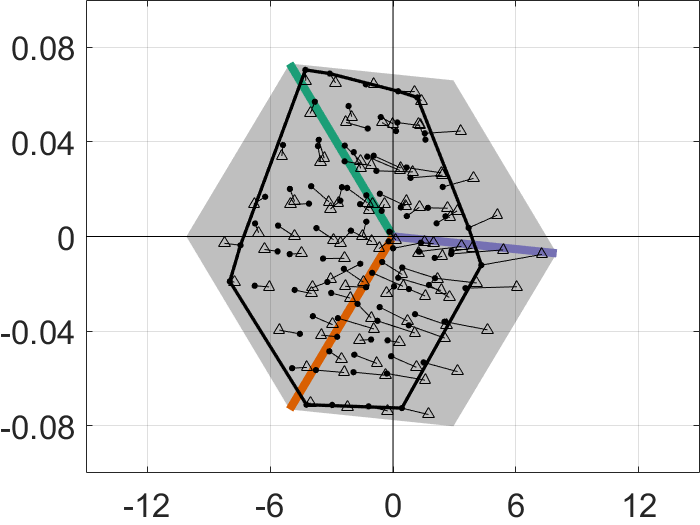
\includegraphics[width=\colWidth]{figures/plots3/s0w0.png}}; %\fill[blue] (0,0) circle (2pt);
&
\node[style={anchor=center}] {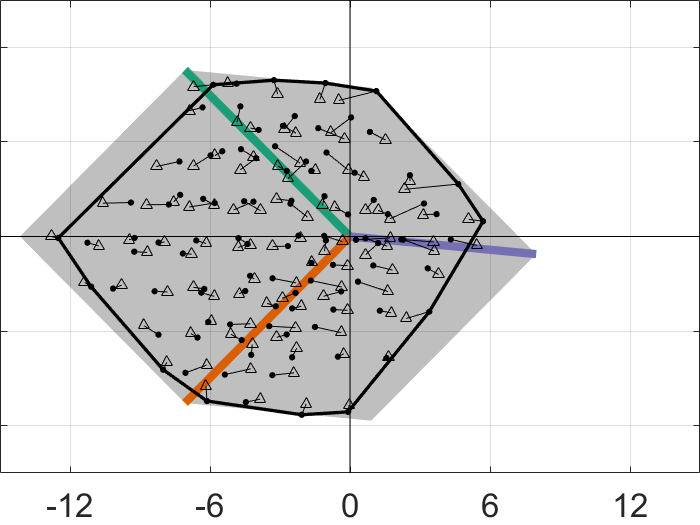
\includegraphics[width=\colWidth]{figures/plots3/s5w0.png}}; %\fill[blue] (0,0) circle (2pt);
&
\node[style={anchor=center}] {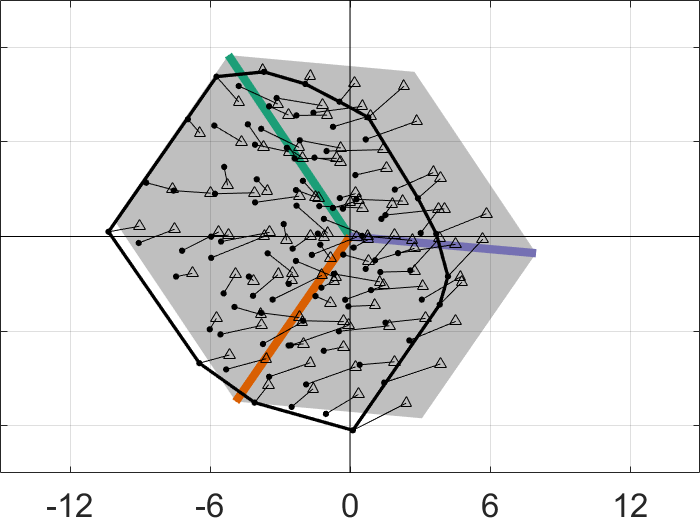
\includegraphics[width=\colWidth]{figures/plots3/s0w20.png}}; %\fill[blue] (0,0) circle (2pt);
&
\node[style={anchor=center}] {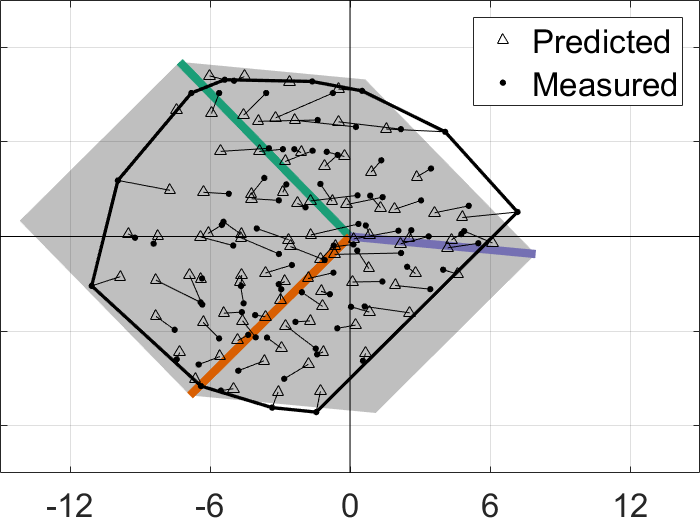
\includegraphics[width=\colWidth]{figures/plots3/s5w20.png}}; %\fill[blue] (0,0) circle (2pt);

\\

& \node (xlabel1) {Force, $F^{\hat{z}_e}$ (N)}; & \node (xlabel2) {Force, $F^{\hat{z}_e}$ (N)}; & \node (xlabel3) {Force, $F^{\hat{z}_e}$ (N)}; & \node (xlabel4) {Force, $F^{\hat{z}_e}$ (N)};

\\
};
\end{tikzpicture}

\caption{For four different deformed configurations (top row), we compare the predicted and the measured forces for the parallel combination of three FREEs (bottom row). 
Data points corresponding to the same input pressures are connected by a thin line.
The data is overlaid on top of the theoretical force zonotopes (grey areas) for each of the four configurations.
Identical colors indicate correspondence between the three FREEs and the resulting force/torque directions.}
\label{fig:results}
\end{figure*}






% & \node (a) {(a)}; & \node (b) {(b)}; & \node (c) {(c)}; & \node (d) {(d)};


For comparison, the measured forces are superimposed over the force zonotope generated by our model in Fig.~\ref{fig:results}a-~\ref{fig:results}d.
To quantify the accuracy of the model, we defined the error at the $j^{th}$ evaluation point as the difference between the modeled and measured forces
\begin{align}
%    \vec{e}_j &= \left( {\vec{\zeta}_{\,\text{mod}}} - {\vec{\zeta}_{\,\text{emp}}} \right)_j
%    e_j &= \left( F/M_{\,\text{mod}} - F/M_{\,\text{emp}} \right)_j
    e^F_j &= \left( F^{\hat{z}_e}_{\text{pred}, j} - F^{\hat{z}_e}_{\text{meas}, j} \right) \\
    e^M_j &= \left( M^{\hat{z}_e}_{\text{pred}, j} - M^{\hat{z}_e}_{\text{meas}, j} \right)
\end{align}
and evaluated the error across all $N = 125$ trials of a given end effector configuration using the following metrics:
\begin{align}
    \text{RMSE} &= \sqrt{ \frac{\sum_{j=1}^{N} e_j^2}{N} } \\
    \text{Max Error} &= \max \{ \left| e_j \right| : j = 1, ... , N \}
\end{align}
As shown in Table \ref{table:RMSE}, the RMSE is less than \unit[1.2]{N} (\unit[${7 \times 10^{-3}}$]{Nm}), and the maximum error is less than \unit[3]{N}  (\unit[${16 \times 10^{-3}}$]{Nm}) across all configurations.

\begin{table}[H]
\centering
\caption{Root-mean-square error and maximum error}
\begin{tabular}{|c || c | c | c | c|}
    \hline
     \rule{0pt}{2ex} \textbf{Displacement} & \multicolumn{2}{c |}{\textbf{RMSE}} & \multicolumn{2}{c |}{\textbf{Max Error}} \\ \cline{2-5}
     \rule{0pt}{2ex} (mm, $^\circ$) & F (N) & M (Nm) & F (N) & M (Nm) \\
     \hline
     0, 0 & 1.13 & $3.8 \times 10^{-3}$ & 2.96 & $7.8 \times 10^{-3}$ \\
     5, 0 & 0.74 & $3.2 \times 10^{-3}$ & 2.31 & $7.4 \times 10^{-3}$ \\
     0, 20 & 1.47 & $6.3 \times 10^{-3}$ & 2.52 & $15.6 \times 10^{-3}$\\
     5, 20 & 1.18 & $4.6 \times 10^{-3}$ & 2.85 & $12.4 \times 10^{-3}$ \\  \hline
\end{tabular}
\label{table:RMSE}
\end{table}

\begin{figure}
    \centering
    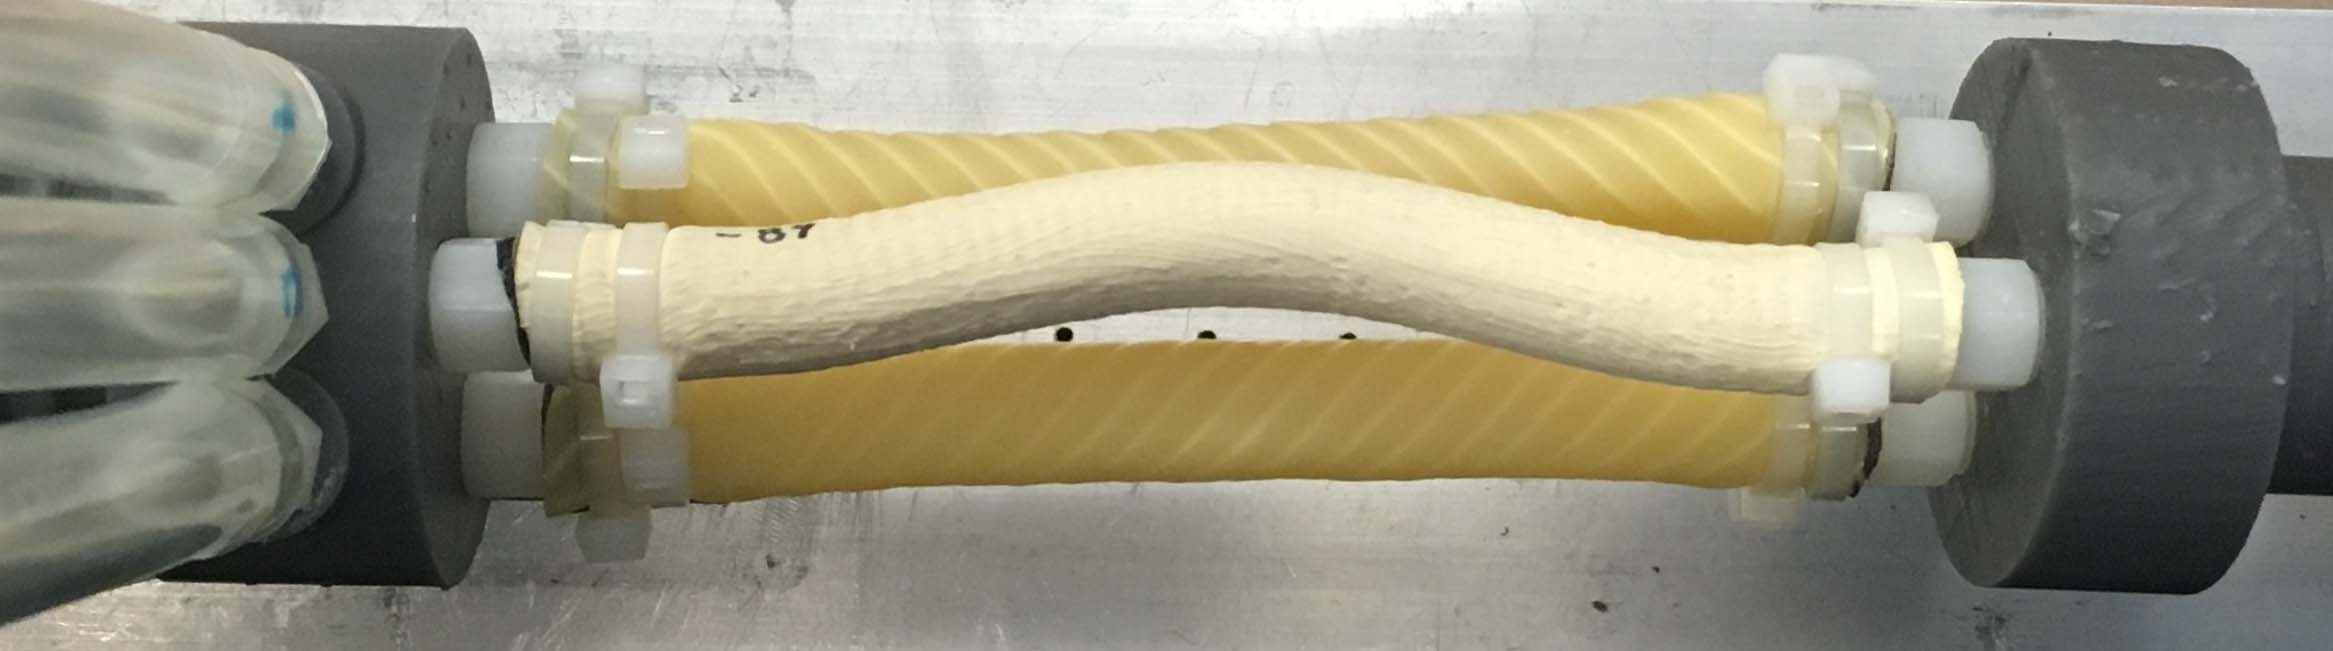
\includegraphics[width=\linewidth]{figures/photos/buckling.jpg}
    \caption{At high fluid pressure the FREE with fiber angle of $-85^\circ$ started to buckle.  This effect was less pronounced when the system was extended along the $z$-axis.}
    \label{fig:buckling}
\end{figure}

%Experimental precision was limited by unmodeled material defects in the FREEs, as well as sensor inaccuracy. While the commercial force and moment sensors used have a quoted accuracy of 0.02\% for the force sensor and 0.2\% for the moment sensor (LoadStar Sensors, 2015), a drifting of up to 0.5 N away from zero was noticed on the force sensor during testing.

It should be noted, that throughout the experiments, the FREE with a fiber angle of $-85^\circ$ exhibited noticeable buckling behavior at pressures above $\approx$ \unit[50]{kPa} (Fig.~\ref{fig:buckling}). 
This behavior was more pronounced during testing in the non-extended configurations (Fig.~\ref{fig:results}a~and~\ref{fig:results}c). 
The buckling might explain the noticeable leftward offset of many of the points in Fig.~\ref{fig:results}a and Fig.~\ref{fig:results}c, since it is reasonable to assume that buckling reduces the efficacy of of the FREE to exert force in the direction normal to the force sensor. 

\begin{figure}
    \centering
    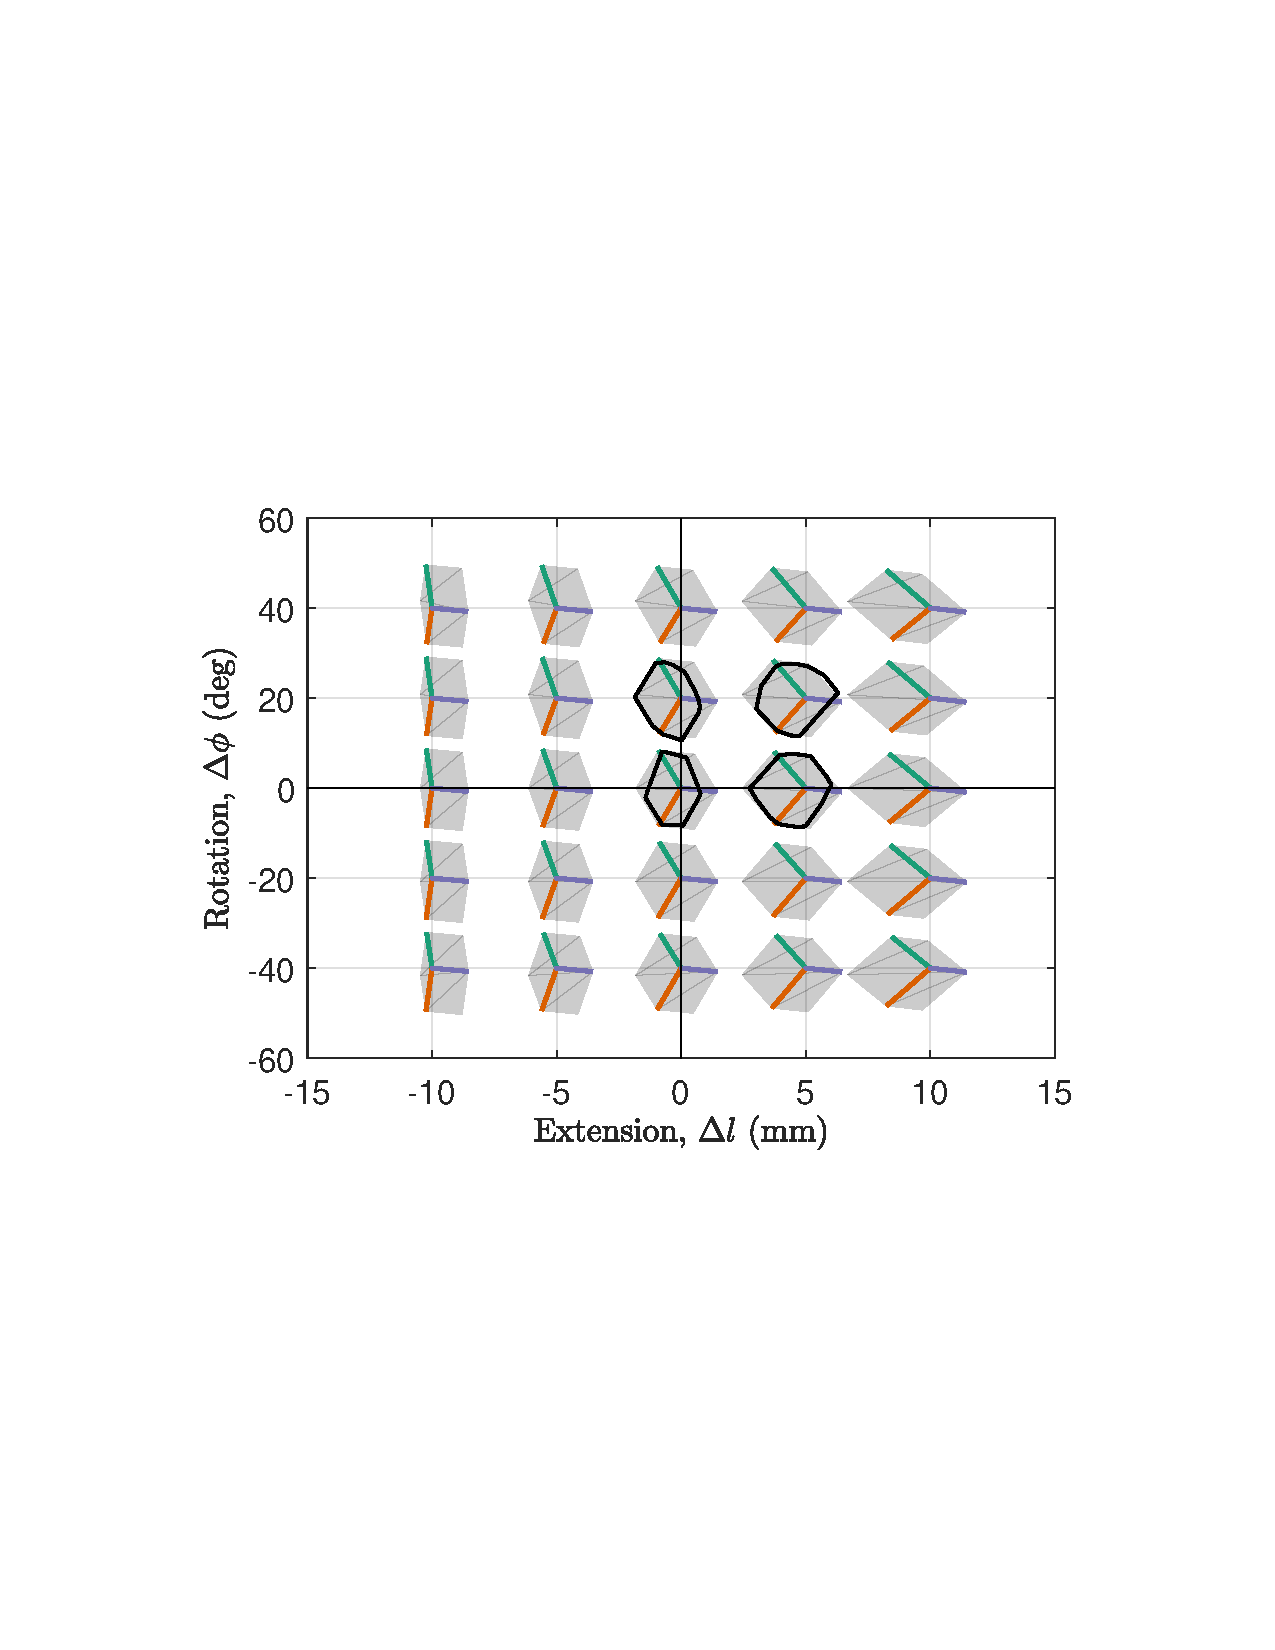
\includegraphics[width=\linewidth]{figures/zntp_vs_x4.pdf}
    \caption{A visualization of how the \emph{force zonotope} of the parallel combination of three FREEs (see Fig.~\ref{fig:rig}) changes as a function of the end effector state $x$. One can observe that the change in the zonotope ultimately limits the work-space of such a system.  In particular the zonotope will collapse for compressions of more than \unit[-10]{mm}.  For \revcomment{2.5}{scale and comparison, the convex hulls of the measured points from Fig.~\ref{fig:results}} are superimposed upon their corresponding zonotope at the configurations that were evaluated experimentally.}
    % \marginnote{\#2.5}
    \label{fig:zntp_vs_x}
\end{figure}















































%%%%%%%%%%%%%%%%%%%%%%%%%%%%%%%%%%%%%%%%%%%%%%%%%%%%%%%%%%%%%%%%%%%%%%%%%%%%%%%%%%%%%%%%%%%
\begin{comment}
From Equations \ref{eq:Z} and \ref{eq:zeta} the predicted force at the end effector is given by
\begin{align}
    \vec{\zeta}(\vec{q}, \vec{P}) &= \sum_{i=1}^3 \bar{\mathcal{D}}_i \left( {\bar{J}_V}_i^T(\vec{q_i}) P_i + \vec{Z}_i^{\text{elast}} (\vec{q_i}) \right) \\
    &= \underbrace{\sum_{i=1}^3 \bar{\mathcal{D}}_i {\bar{J}_V}_i^T(\vec{q_i}) P_i}_{\vec{\zeta}^{\,\text{fiber}} (\vec{q}, \vec{P})} + \underbrace{\sum_{i=1}^3 \bar{\mathcal{D}}_i \vec{Z}_i^{\text{elast}} (\vec{q_i})}_{\vec{\zeta}^{\text{elast}} (\vec{q})} \\
%     &= \vec{\zeta}^{\,\text{fiber}} (\vec{q}, \vec{P}) + \vec{\zeta}^{\text{elast}} (\vec{q})
\end{align}




Furthermore, we assumed that all of the FREEs exerted forces along/about the z-axis, which we enforced this assumption by positioning the FREEs as close together as possible, and imposing physical constraints

Since we only measure forces/moments along/about the end effector z-axis, in our model of the experimental system we assume there is no offset. 


We can isolate the elastomer force component by setting the pressure equal to zero
\begin{align}
    \vec{\zeta}(\vec{q}, 0) &= 0 + \vec{\zeta}^{\text{elast}} (\vec{q})
\end{align}
Then, we can isolate the fiber force component by subtracting the elastomer force component from the total measured force
\begin{align}
    \vec{\zeta}^{\,\text{fiber}} (\vec{q}, \vec{P})  &= \vec{\zeta}(\vec{q}, \vec{P}) - \vec{\zeta}(\vec{q}, 0) \\
    or \\
    \vec{\zeta}^{\,\text{fiber}}_{\text{emp}} (\vec{q}, \vec{P})  &= \vec{\zeta}_{\text{emp}}(\vec{q}, \vec{P}) - \vec{\zeta}_{\text{emp}}(\vec{q}, 0)
\end{align} 

\begin{align}
    \vec{\zeta}^{\text{fiber}}_{\text{mod}} (\vec{q}, \vec{P}) &= \sum_{i=1}^n \bar{\mathcal{D}}_i {\bar{J}_V}_i^T(\vec{q_i}) P_i \\
    \vec{\zeta}^{\,\text{fiber}}_{\text{emp}} (\vec{q}, \vec{P})  &= \vec{\zeta}_{\text{emp}}(\vec{q}, \vec{P}) - \vec{\zeta}_{\text{emp}}(\vec{q}, 0)
\end{align}
 
\end{comment}



%% OLD VERSION BELOW THIS LINE %%%%%%%%%%%%%%%%%%%%%%%%%%%%%%%%%%%%%%%%%%%%%%%%%%%%%%%%%%%%%%%%%%%%%%%%%%%%%%%%%%
\begin{comment}
To validate the force polygon derivation we compared the model predicted equilibrium positions to those measured on a physical system. We built a test platform consisting of 4 FREEs in a parallel configuration like the one shown in Fig. \ref{fig:testPlatform}, then measured the equilibrium orientation of the end effector for several combination of input pressure. Since the position of the origin of the end effector was fixed in space by a rigid structure, to fully characterize its position we only needed to measure its orientation using a inertial measurement unit (IMU).

\begin{figure}
    \centering
    \begin{tabular}{c c}
        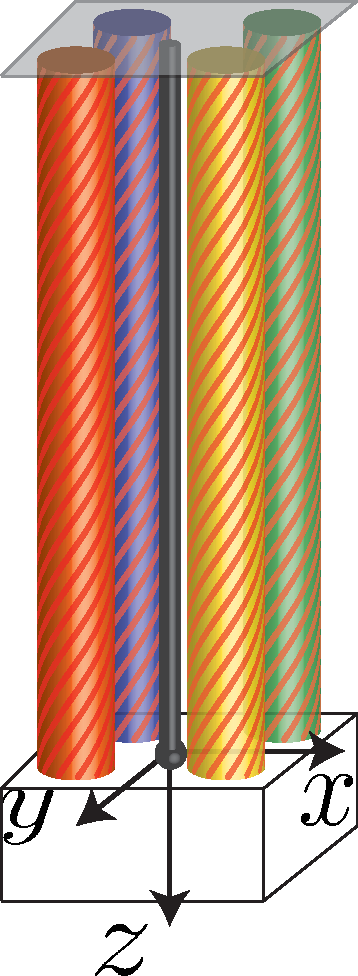
\includegraphics[width=0.2\linewidth]{figures/testPlatform-v2.pdf} &
        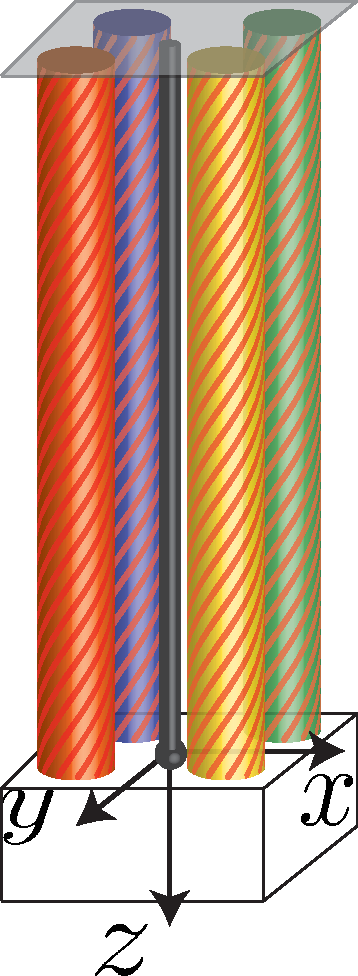
\includegraphics[width=0.2\linewidth]{figures/testPlatform-v2.pdf}
    \end{tabular}
    \caption{The parallel setup used for the experiment has a rod constraining the position of the origin of the end effector. The rod is a connected to the end effector by a ball joint so as not to constrain its orientation. (May replace with 3D dimensional drawing from solidworks, and will have photo of actual test rig adjacent).}
    \label{fig:testPlatform}
\end{figure}




\subsection{Relationship between FREE and End Effector States}
In general, the state of each FREE in a parallel combination $\vec{q}_i$ can be expressed as a function of the end effector state $\vec{x}$ under sufficient assumptions. In our experimental case, we assume that the central axis of each FREE lies entirely on a cylindrical manifold of radius $\rho = ??$ centered about the central constraint rod. Under this assumption, the following relationship emerges
\begin{align}
    \vec{q}_{i}(\vec{x}) &= \begin{bmatrix} -L + \sqrt{(L - s_{\theta} d_{i}^x + c_{\theta} s_{\psi} d_{i}^y)^2 + ({d_{i}^x}^2 + {d_{i}^{y}}^2) \phi^2} \\ \phi \end{bmatrix}
\end{align}
where $L$ is the length of the central constraint rod, and $\vec{d}_i = \bmx d_i^x & d_i^y & d_i^z \emx$ is the attachment point of the $i^{th}$ FREE in end effector coordinates. We use this expression in equation \ref{eq:Zi} to calculate the force generated by each FREE, numerically solve Equation \ref{eq:equil} to find equilibrium points of the experimental model, then compare them to those of the physical system under identical steady state inputs.



\subsection{System Identification of FREE Elastomer Parameters}





\subsection{Experimental Procedure}

\end{comment}




\begin{comment}
The experimental error can be attributed to two sources; model inaccuracy and sensor 

Sources of Error
-Sensor preloading
-Misalignment of FREEs
-Sensor noise
-

Shortcomings of Model
-Model cannot handle buckling
-The end effector displacements were intentionally chosen to avoid configurations where buckling might occur.
\end{comment}